\documentclass[aspectratio=169,11pt]{beamer}
\usepackage[utf8]{inputenc}
\usepackage[T1]{fontenc}
\usepackage[english]{babel}
\usetheme{Madrid}
\usecolortheme{whale}
\definecolor{uddblue}{HTML}{1F4E79}
\definecolor{uddlight}{HTML}{2E86C1}
\setbeamercolor{structure}{fg=uddblue}
\setbeamercolor{frametitle}{bg=uddblue,fg=white}
\setbeamercolor{title}{bg=uddblue,fg=white}
\setbeamercolor{block title}{bg=uddblue,fg=white}
\setbeamercolor{block body}{bg=uddblue!10}
\setbeamercolor{item}{fg=uddblue}
\usepackage{amsmath,amssymb}
\usepackage{graphicx}
\usepackage{booktabs}
\usepackage{listings}
\usepackage{tikz}
\usetikzlibrary{shapes,arrows,positioning,calc}
\lstset{language=R,basicstyle=\ttfamily\scriptsize,keywordstyle=\color{uddblue}\bfseries,commentstyle=\color{gray},stringstyle=\color{uddlight},backgroundcolor=\color{uddblue!5},frame=single,rulecolor=\color{uddblue!30},breaklines=true,showstringspaces=false,extendedchars=true}
\graphicspath{{figuras/}}
\titlegraphic{
\includegraphics[height=1.2cm]{logo_gobierno.png}}
\institute[CICS --- UDD]{Doctorado en Ciencias de la Complejidad Social --- CICS, UDD}
\newcommand{\highlight}[1]{\textcolor{uddlight}{\bfseries #1}}

\title{Pruebas de Hip\'otesis}
\subtitle{Sesi\'on 1 --- Fundamentos y Aplicaciones}
\author[A. Ag\"uero]{Amaru Ag\"uero}
\date{23 de marzo de 2026}

\begin{document}

% ============================================================================
% SLIDE 1: Title Slide
% ============================================================================
\begin{frame}[plain]
  \titlepage
\end{frame}

% ============================================================================
% SLIDE 2: Agenda
% ============================================================================
\begin{frame}
  \frametitle{Agenda de la Sesi\'on}
  \begin{itemize}
    \setlength{\itemsep}{4pt}
    \item L\'ogica y fundamentos de las pruebas de hip\'otesis
    \item Hip\'otesis nula ($H_0$) e hip\'otesis alternativa ($H_1$)
    \item Estad\'istico de prueba y valor-p: interpretaci\'on visual
    \item Matriz de decisi\'on: Errores Tipo I y II
    \item Prueba t de una muestra: concepto y aplicaci\'on
    \item Prueba t de dos muestras: comparaci\'on de medias
    \item Pruebas de proporciones y sus aplicaciones
    \item Prueba chi-cuadrado de independencia
    \item Potencia estad\'istica y tama\~no de muestra
    \item Implementaci\'on en R
  \end{itemize}
\end{frame}

% ============================================================================
% SLIDE 3: Que es una Prueba de Hipotesis
% ============================================================================
\begin{frame}
  \frametitle{?`Qu\'e es una Prueba de Hip\'otesis?}
  \begin{block}{Definici\'on}
    Un \highlight{procedimiento estad\'istico} que permite evaluar si una afirmaci\'on sobre
    una poblaci\'on es consistente con la evidencia muestral recolectada.
  \end{block}
  \pause
  \begin{itemize}
    \setlength{\itemsep}{4pt}
    \item Basada en la \textbf{l\'ogica del razonamiento por contradicci\'on}
    \item Utilizamos \textit{muestras} para hacer inferencias sobre \textit{poblaciones}
    \item Controlamos el riesgo de cometer errores estad\'isticos
    \item Fundamentada en la teor\'ia de probabilidades
  \end{itemize}
  \pause
  \vspace{0.2cm}
  \textit{Idea central:} Asumir que no hay efecto ($H_0$) y preguntar: ?`qu\'e tan probable es observar nuestros datos si eso fuera cierto?
\end{frame}

% ============================================================================
% SLIDE 4: H0 y H1
% ============================================================================
\begin{frame}
  \frametitle{Hip\'otesis Nula ($H_0$) e Hip\'otesis Alternativa ($H_1$)}
  \small
  \begin{columns}[T]
    \column{0.5\textwidth}
    \textbf{Hip\'otesis Nula ($H_0$):}
    \begin{itemize}
      \setlength{\itemsep}{3pt}
      \item Afirmaci\'on de \textit{``no efecto''} o \textit{``no diferencia''}
      \item Punto de partida del an\'alisis
      \item Asumimos que es verdadera a menos que haya evidencia contraria
      \item Ej: $\mu = 100$
    \end{itemize}

    \column{0.5\textwidth}
    \textbf{Hip\'otesis Alternativa ($H_1$):}
    \begin{itemize}
      \setlength{\itemsep}{3pt}
      \item Lo que queremos \textit{demostrar} con los datos
      \item Contradice a $H_0$
      \item Puede ser unilateral o bilateral
      \item Ej: $\mu \neq 100$
    \end{itemize}
  \end{columns}

  \vspace{0.4cm}
  \begin{exampleblock}{Ejemplo en Ciencias Sociales}
    $H_0$: El ingreso promedio de hombres y mujeres es igual \\
    $H_1$: El ingreso promedio difiere entre hombres y mujeres
  \end{exampleblock}
\end{frame}

% ============================================================================
% SLIDE 5: Proceso de Prueba
% ============================================================================
\begin{frame}
  \frametitle{Proceso de Prueba de Hip\'otesis}
  \small
  \begin{center}
    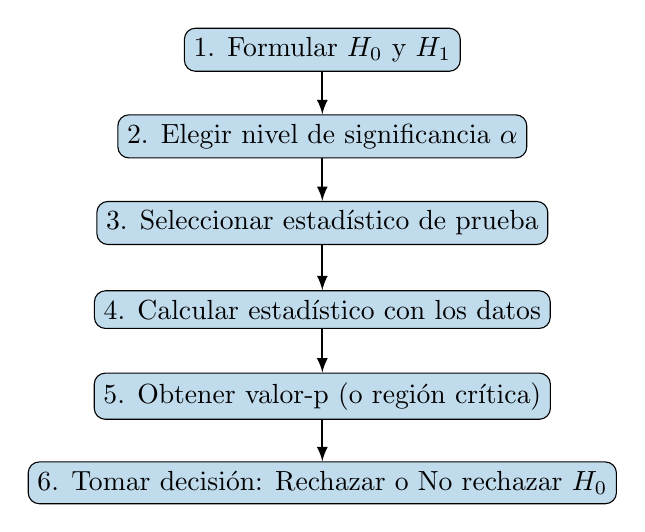
\begin{tikzpicture}[node distance=1.1cm, scale=0.9]
      \node (step1) [draw, rectangle, rounded corners, fill=uddlight!30] {1. Formular $H_0$ y $H_1$};
      \node (step2) [draw, rectangle, rounded corners, fill=uddlight!30, below of=step1] {2. Elegir nivel de significancia $\alpha$};
      \node (step3) [draw, rectangle, rounded corners, fill=uddlight!30, below of=step2] {3. Seleccionar estad\'istico de prueba};
      \node (step4) [draw, rectangle, rounded corners, fill=uddlight!30, below of=step3] {4. Calcular estad\'istico con los datos};
      \node (step5) [draw, rectangle, rounded corners, fill=uddlight!30, below of=step4] {5. Obtener valor-p (o regi\'on cr\'itica)};
      \node (step6) [draw, rectangle, rounded corners, fill=uddlight!30, below of=step5] {6. Tomar decisi\'on: Rechazar o No rechazar $H_0$};

      \draw [-latex, thick] (step1) -- (step2);
      \draw [-latex, thick] (step2) -- (step3);
      \draw [-latex, thick] (step3) -- (step4);
      \draw [-latex, thick] (step4) -- (step5);
      \draw [-latex, thick] (step5) -- (step6);
    \end{tikzpicture}
  \end{center}
  \vspace{-0.1cm}
  \textit{Nota:} El nivel de significancia $\alpha$ t\'ipicamente es 0.05 (5\%).
\end{frame}

% ============================================================================
% SLIDE 6: Estadistico de prueba y valor-p
% ============================================================================
\begin{frame}
  \frametitle{Estad\'istico de Prueba y Valor-p}
  \small
  \begin{block}{Estad\'istico de prueba}
    Transforma los datos en un \textbf{n\'umero \'unico} que mide cu\'an lejos est\'an de lo esperado bajo $H_0$.
    \[
      t = \frac{\text{estimaci\'on} - \text{valor bajo } H_0}{\text{error est\'andar}} = \frac{\bar{x} - \mu_0}{s / \sqrt{n}}
    \]
  \end{block}

  \pause
  \vspace{0.2cm}
  \begin{block}{Valor-p}
    Probabilidad de obtener un resultado \textbf{tan extremo o m\'as} que el observado, \textit{suponiendo que $H_0$ es cierta}.
  \end{block}

  \vspace{0.2cm}
  \textbf{Regla de decisi\'on:}
  \begin{itemize}
    \item Si $p < \alpha$ (t\'ipicamente 0.05) $\to$ \highlight{Rechazar $H_0$}
    \item Si $p \geq \alpha$ $\to$ \textbf{No rechazar $H_0$}
  \end{itemize}
\end{frame}

% ============================================================================
% SLIDE 7: Valor-p visual (NUEVA FIGURA)
% ============================================================================
\begin{frame}
  \frametitle{Interpretaci\'on Visual del Valor-p}
  \begin{center}
    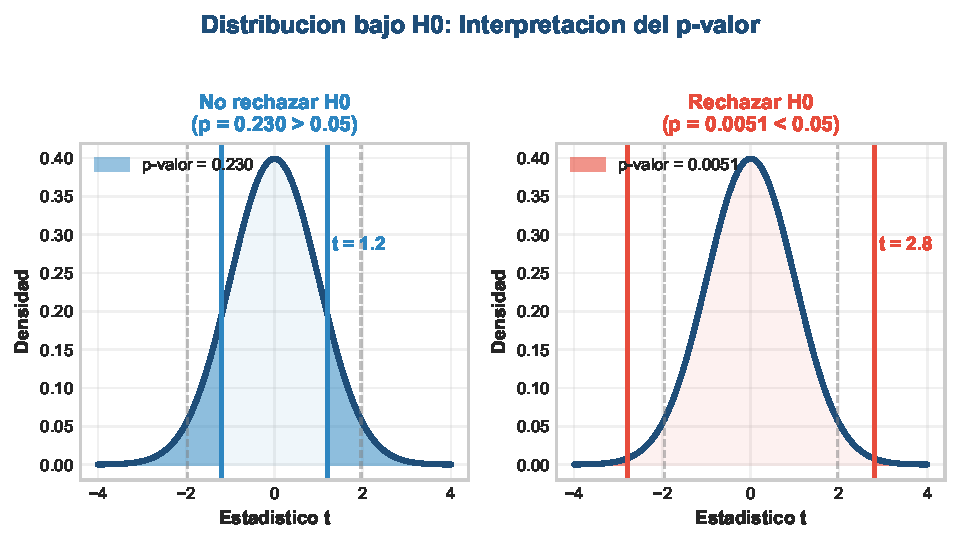
\includegraphics[height=0.78\textheight]{h0_h1_pvalor.pdf}
  \end{center}
  \vspace{-0.2cm}
  {\scriptsize El \'area sombreada es el \textbf{valor-p}: a menor \'area, mayor evidencia contra $H_0$.}
\end{frame}

% ============================================================================
% SLIDE 8: Regiones de rechazo
% ============================================================================
\begin{frame}
  \frametitle{Regiones de Rechazo: Prueba Bilateral}
  \begin{center}
    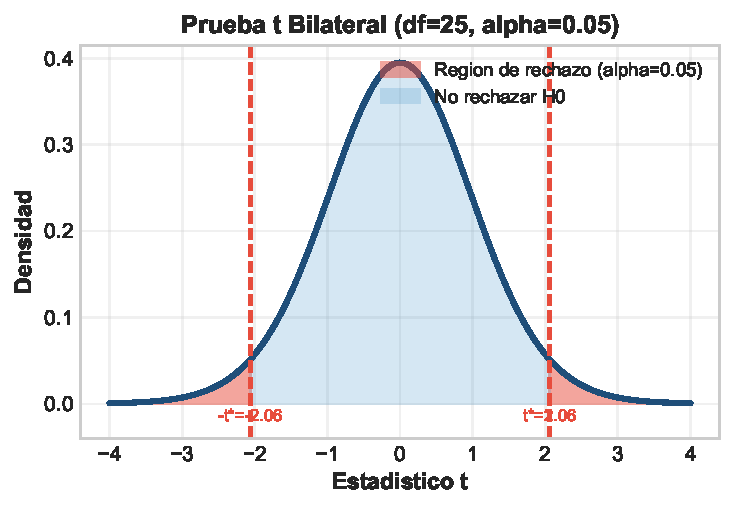
\includegraphics[height=0.78\textheight]{distribucion_prueba_t.pdf}
  \end{center}
\end{frame}

% ============================================================================
% SLIDE 9: Prueba t de una muestra --- Concepto
% ============================================================================
\begin{frame}
  \frametitle{Prueba t de una Muestra: Concepto}
  \small
  \begin{block}{Objetivo}
    Comparar la media de una muestra contra un valor hipot\'etico $\mu_0$ de la poblaci\'on.
  \end{block}

  \textbf{Estad\'istico de prueba:}
  \[
    t = \frac{\bar{x} - \mu_0}{s / \sqrt{n}}
  \]
  donde: $\bar{x}$ = media muestral, $s$ = desviaci\'on est\'andar, $n$ = tama\~no de muestra

  \vspace{0.2cm}
  \textbf{Supuestos:}
  \begin{itemize}
    \setlength{\itemsep}{2pt}
    \item Muestra aleatoria de la poblaci\'on
    \item Variable distribuida aproximadamente normal
    \item Observaciones independientes
  \end{itemize}

  \textbf{Grados de libertad:} $\nu = n - 1$
\end{frame}

% ============================================================================
% SLIDE 10: Prueba t de una muestra --- Ejemplo
% ============================================================================
\begin{frame}
  \frametitle{Prueba t de una Muestra: Ejemplo Pr\'actico}
  \small
  \begin{exampleblock}{Caso: Edad promedio de participantes}
    Se desea probar si la edad promedio de participantes en un programa de capacitaci\'on
    es diferente de 35 a\~nos.
  \end{exampleblock}

  \textbf{Datos:} $n = 25$, $\bar{x} = 37.5$, $s = 8.2$ a\~nos

  \vspace{0.2cm}
  \textbf{Hip\'otesis:}
  \begin{itemize}
    \item $H_0: \mu = 35$ \quad (la edad promedio es 35 a\~nos)
    \item $H_1: \mu \neq 35$ \quad (la edad promedio difiere de 35 a\~nos)
    \item $\alpha = 0.05$
  \end{itemize}

  \vspace{0.2cm}
  \textbf{C\'alculo:}
  \[
    t = \frac{37.5 - 35}{8.2 / \sqrt{25}} = \frac{2.5}{1.64} \approx 1.52
  \]

  Con $\nu = 24$, $t_{0.025} = 2.064$. Como $|1.52| < 2.064$, \highlight{no rechazamos} $H_0$.
\end{frame}

% ============================================================================
% SLIDE 11: Prueba t de dos muestras --- Concepto
% ============================================================================
\begin{frame}
  \frametitle{Prueba t de Dos Muestras: Concepto}
  \small
  \begin{block}{Objetivo}
    Comparar si las medias de dos grupos independientes son iguales.
  \end{block}

  \textbf{Hip\'otesis est\'andar:}
  \begin{itemize}
    \item $H_0: \mu_1 = \mu_2$ (las medias son iguales)
    \item $H_1: \mu_1 \neq \mu_2$ (las medias difieren)
  \end{itemize}

  \vspace{0.2cm}
  \textbf{Estad\'istico (varianzas iguales):}
  \[
    t = \frac{\bar{x}_1 - \bar{x}_2}{s_p \sqrt{\frac{1}{n_1} + \frac{1}{n_2}}}
  \]
  donde $s_p$ es la desviaci\'on est\'andar combinada (pooled).

  \vspace{0.2cm}
  \textbf{Grados de libertad:} $\nu = n_1 + n_2 - 2$
\end{frame}

% ============================================================================
% SLIDE 12: Prueba t de dos muestras --- Ejemplo
% ============================================================================
\begin{frame}
  \frametitle{Prueba t de Dos Muestras: Ejemplo}
  \small
  \begin{exampleblock}{Caso: Diferencia de ingresos por g\'enero}
    Comparar si el ingreso mensual promedio difiere entre hombres y mujeres.
  \end{exampleblock}

  \textbf{Datos:}
  \begin{itemize}
    \setlength{\itemsep}{2pt}
    \item Grupo 1 (Hombres): $n_1 = 50$, $\bar{x}_1 = \$2500$, $s_1 = \$450$
    \item Grupo 2 (Mujeres): $n_2 = 45$, $\bar{x}_2 = \$2200$, $s_2 = \$520$
  \end{itemize}

  \vspace{0.2cm}
  \textbf{Hip\'otesis:} $H_0: \mu_H = \mu_M$ \quad vs \quad $H_1: \mu_H \neq \mu_M$ \quad ($\alpha = 0.05$)

  \vspace{0.2cm}
  \textbf{C\'alculo resumido:} $s_p \approx 487$, $t \approx 2.96$, $p\text{-valor} < 0.01$

  \vspace{0.2cm}
  \highlight{Conclusi\'on:} Rechazamos $H_0$ --- hay evidencia de diferencia significativa de ingresos.
\end{frame}

% ============================================================================
% SLIDE 13: Pruebas de proporciones
% ============================================================================
\begin{frame}
  \frametitle{Pruebas de Proporciones}
  \small
  \begin{block}{Objetivo}
    Probar hip\'otesis sobre proporciones (porcentajes) en una o dos poblaciones.
  \end{block}

  \textbf{Prueba de una proporci\'on:}
  \[
    z = \frac{\hat{p} - p_0}{\sqrt{\frac{p_0(1-p_0)}{n}}}
  \]

  \textbf{Prueba de dos proporciones:}
  \[
    z = \frac{\hat{p}_1 - \hat{p}_2}{\sqrt{\hat{p}(1-\hat{p})\left(\frac{1}{n_1} + \frac{1}{n_2}\right)}}
  \]

  donde $\hat{p} = \frac{x_1 + x_2}{n_1 + n_2}$ es la proporci\'on combinada.

  \vspace{0.2cm}
  \textbf{Supuestos:} $np_0 \geq 5$ y $n(1-p_0) \geq 5$ (aproximaci\'on normal)
\end{frame}

% ============================================================================
% SLIDE 14: Chi-cuadrado de independencia
% ============================================================================
\begin{frame}
  \frametitle{Prueba Chi-cuadrado de Independencia}
  \small
  \begin{block}{Objetivo}
    Determinar si dos variables categ\'oricas son independientes.
  \end{block}

  \textbf{Hip\'otesis:}
  \begin{itemize}
    \item $H_0$: Las variables son independientes
    \item $H_1$: Las variables est\'an asociadas
  \end{itemize}

  \vspace{0.2cm}
  \textbf{Estad\'istico de prueba:}
  \[
    \chi^2 = \sum_{i,j} \frac{(O_{ij} - E_{ij})^2}{E_{ij}}
  \]
  donde $O_{ij}$ = frecuencia observada, $E_{ij} = \frac{(\text{total fila}_i)(\text{total col}_j)}{n}$

  \vspace{0.2cm}
  \textbf{Grados de libertad:} $\nu = (r-1)(c-1)$ \quad \textbf{Supuesto:} $E_{ij} \geq 5$ en al menos 80\% de celdas
\end{frame}

% ============================================================================
% SLIDE 15: Ejemplo chi-cuadrado
% ============================================================================
\begin{frame}
  \frametitle{Ejemplo: Chi-cuadrado de Independencia}
  \small
  \begin{exampleblock}{Caso: Relaci\'on entre educaci\'on y participaci\'on pol\'itica}
    ?`Existe asociaci\'on entre nivel educativo y participaci\'on en elecciones?
  \end{exampleblock}

  \vspace{0.2cm}
  \begin{center}
    \begin{tabular}{l|cc|c}
      \toprule
      & \textbf{Vot\'o} & \textbf{No Vot\'o} & \textbf{Total} \\
      \midrule
      \textbf{Edu. Superior} & 180 & 20 & 200 \\
      \textbf{Edu. Secundaria} & 150 & 50 & 200 \\
      \textbf{Edu. Primaria} & 90 & 110 & 200 \\
      \midrule
      \textbf{Total} & 420 & 180 & 600 \\
      \bottomrule
    \end{tabular}
  \end{center}

  \vspace{0.2cm}
  $\chi^2 \approx 96.43$, $\nu = 2$, $p\text{-valor} < 0.001$

  \highlight{Conclusi\'on:} Existe asociaci\'on significativa entre educaci\'on y participaci\'on.
\end{frame}

% ============================================================================
% SLIDE 16: Distribucion chi-cuadrado (figura)
% ============================================================================
\begin{frame}
  \frametitle{Distribuci\'on Chi-Cuadrado}
  \begin{center}
    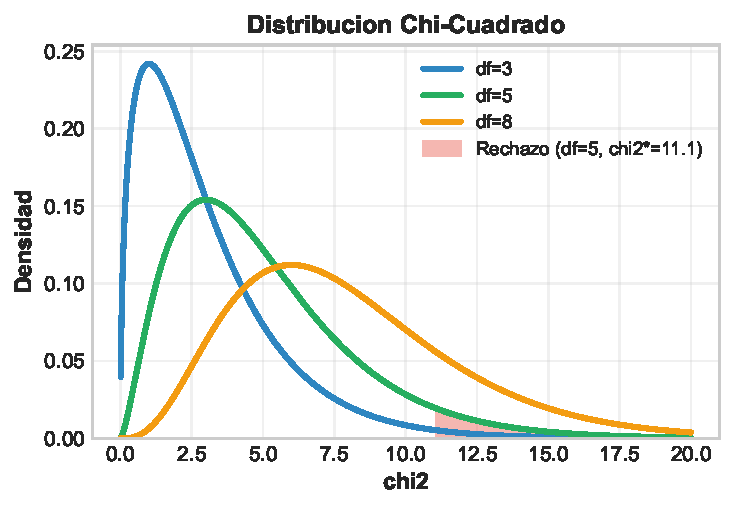
\includegraphics[height=0.78\textheight]{chi_cuadrado.pdf}
  \end{center}
\end{frame}

% ============================================================================
% SLIDE 17: Matriz de decision (NUEVA FIGURA)
% ============================================================================
\begin{frame}
  \frametitle{Matriz de Decisi\'on: Errores Tipo I y II}
  \begin{center}
    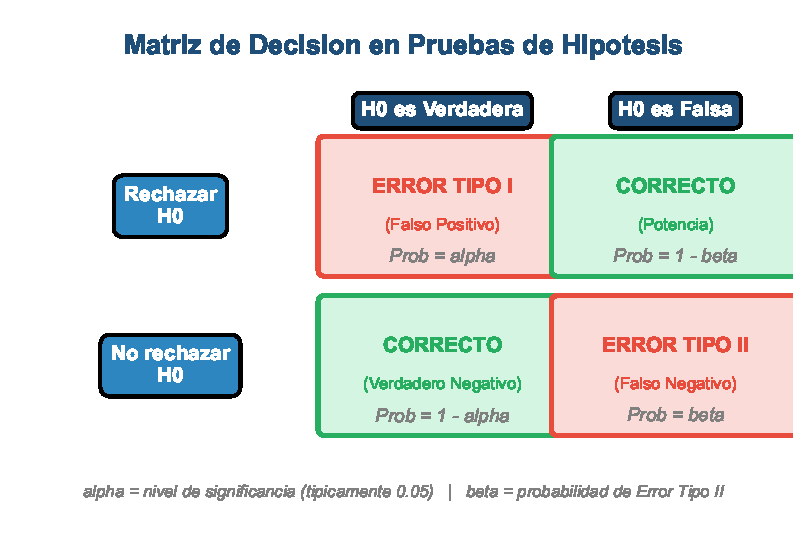
\includegraphics[height=0.78\textheight]{matriz_decision.pdf}
  \end{center}
\end{frame}

% ============================================================================
% SLIDE 18: Errores tipo I y II --- Explicacion
% ============================================================================
\begin{frame}
  \frametitle{Errores Tipo I y II: Detalle}
  \small
  \begin{itemize}
    \setlength{\itemsep}{5pt}
    \item \textbf{Error Tipo I ($\alpha$):} Rechazar $H_0$ cuando es verdadera (``falso positivo'').
      El investigador controla este riesgo fijando $\alpha$ (e.g., 0.05).

    \item \textbf{Error Tipo II ($\beta$):} No rechazar $H_0$ cuando es falsa (``falso negativo'').
      Depende del tama\~no de muestra, el tama\~no de efecto y la variabilidad.

    \item \textbf{Trade-off:} Reducir $\alpha$ (ser m\'as exigente) aumenta $\beta$, y viceversa. La \'unica forma de reducir ambos simult\'aneamente es \textit{aumentar $n$}.
  \end{itemize}

  \vspace{0.3cm}
  \begin{exampleblock}{Analog\'ia: sistema judicial}
    \small
    Error Tipo I = condenar a un inocente (``falso positivo'') \\
    Error Tipo II = absolver a un culpable (``falso negativo'')
  \end{exampleblock}
\end{frame}

% ============================================================================
% SLIDE 19: Errores tipo visualmente (NUEVA FIGURA)
% ============================================================================
\begin{frame}
  \frametitle{Errores Tipo I y II: Vista con Distribuciones}
  \begin{center}
    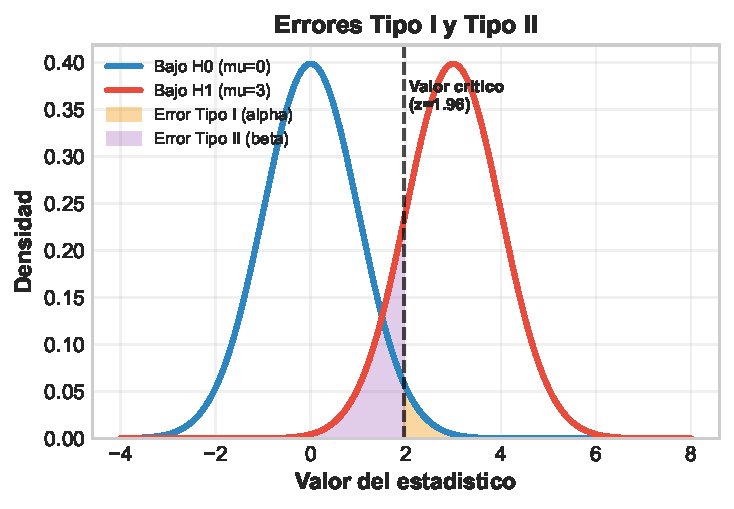
\includegraphics[height=0.78\textheight]{errores_tipo.pdf}
  \end{center}
  \vspace{-0.2cm}
  {\scriptsize Naranja = Error Tipo I ($\alpha$, cola de $H_0$). Morado = Error Tipo II ($\beta$, cuerpo de $H_1$).}
\end{frame}

% ============================================================================
% SLIDE 20: Potencia estadistica
% ============================================================================
\begin{frame}
  \frametitle{Potencia Estad\'istica}
  \begin{block}{Definici\'on}
    La \highlight{potencia} es la probabilidad de rechazar $H_0$ cuando es verdaderamente falsa.
    \[
      \text{Potencia} = 1 - \beta
    \]
  \end{block}

  \vspace{0.3cm}
  \textbf{Factores que afectan la potencia:}
  \begin{itemize}
    \setlength{\itemsep}{3pt}
    \item \textbf{Tama\~no del efecto:} Diferencias m\'as grandes $\to$ mayor potencia
    \item \textbf{Tama\~no de muestra:} Muestras m\'as grandes $\to$ mayor potencia
    \item \textbf{Nivel de significancia $\alpha$:} Mayor $\alpha$ $\to$ mayor potencia (pero m\'as Error Tipo I)
    \item \textbf{Variabilidad:} Menor variabilidad $\to$ mayor potencia
  \end{itemize}

  \vspace{0.2cm}
  \textit{Objetivo t\'ipico:} Dise\~nar estudios con potencia $\geq 0.80$ (80\%).
\end{frame}

% ============================================================================
% SLIDE 21: Potencia figura
% ============================================================================
\begin{frame}
  \frametitle{Potencia vs Tama\~no de Muestra}
  \begin{center}
    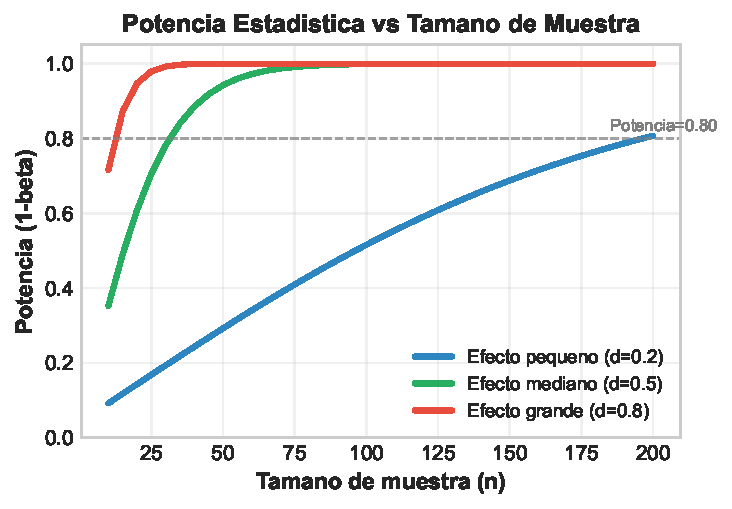
\includegraphics[height=0.78\textheight]{potencia_estadistica.pdf}
  \end{center}
\end{frame}

% ============================================================================
% SLIDE 22: Implementacion en R --- Prueba t
% ============================================================================
\begin{frame}[fragile]
  \frametitle{Implementaci\'on en R: Prueba t}
  \tiny
  \begin{lstlisting}
# Prueba t de una muestra
t.test(edad, mu = 35, alternative = "two.sided")

# Prueba t de dos muestras independientes
t.test(ingreso ~ genero, data = datos,
       var.equal = TRUE, paired = FALSE)

# Prueba t pareada
t.test(antes, despues, paired = TRUE)

# Typical output:
#   t = 1.52, df = 24, p-value = 0.142
#   alternative hypothesis: true mean is not equal to 35
#   95% confidence interval: [32.8, 40.2]
#   sample estimate: mean of x = 37.5
  \end{lstlisting}
\end{frame}

% ============================================================================
% SLIDE 23: Implementacion en R --- Chi-cuadrado y proporciones
% ============================================================================
\begin{frame}[fragile]
  \frametitle{Implementaci\'on en R: M\'as Pruebas}
  \tiny
  \begin{lstlisting}
# Prueba chi-cuadrado de independencia
tabla <- table(educacion, voto)
chisq.test(tabla)

# Proportion test
prop.test(x = 180, n = 200, p = 0.5)

# Prueba de dos proporciones
prop.test(x = c(180, 150), n = c(200, 200))

# Potencia: calcular n necesario para potencia = 0.80
library(pwr)
pwr.t.test(d = 0.5, sig.level = 0.05, power = 0.80, type = "two.sample")
  \end{lstlisting}
\end{frame}

% ============================================================================
% SLIDE 24: Ejercicio practico I
% ============================================================================
\begin{frame}
  \frametitle{Ejercicio Pr\'actico: Parte I}
  \small
  \begin{exampleblock}{Escenario}
    Se tiene un conjunto de datos con 150 participantes en un programa de capacitaci\'on.
    Se recolect\'o informaci\'on sobre: edad, g\'enero, nivel educativo, ingresos antes y despu\'es.
  \end{exampleblock}

  \vspace{0.3cm}
  \textbf{Preguntas:}
  \begin{enumerate}
    \setlength{\itemsep}{5pt}
    \item ?`La edad promedio de participantes es diferente de 40 a\~nos?
    \item ?`Existe diferencia en ingresos iniciales entre hombres y mujeres?
    \item ?`Hay asociaci\'on entre nivel educativo y participaci\'on en actividades?
    \item ?`Aument\'o significativamente el ingreso promedio despu\'es del programa?
  \end{enumerate}

  \vspace{0.2cm}
  \textit{Nota:} Identifique qu\'e prueba corresponde a cada pregunta antes de ver la soluci\'on.
\end{frame}

% ============================================================================
% SLIDE 25: Ejercicio practico II
% ============================================================================
\begin{frame}[fragile]
  \frametitle{Ejercicio Pr\'actico: Soluci\'on en R}
  \tiny
  \begin{lstlisting}
# Cargar datos
datos <- read.csv("capacitacion.csv")

# Question 1: Age different from 40? -> t.test una muestra
t.test(datos$edad, mu = 40)

# Question 2: Income difference by gender -> t.test dos muestras
t.test(ingresos_ini ~ genero, data = datos)

# Question 3: Education-participation association -> chi-cuadrado
tabla <- table(datos$educacion, datos$participacion)
chisq.test(tabla)

# Question 4: Income before vs after -> t.test pareada
t.test(datos$ingresos_antes, datos$ingresos_despues, paired = TRUE)
  \end{lstlisting}
\end{frame}

% ============================================================================
% SLIDE 26: Resumen
% ============================================================================
\begin{frame}
  \frametitle{Resumen de Conceptos Clave}
  \small
  \begin{itemize}
    \setlength{\itemsep}{5pt}
    \item Las pruebas de hip\'otesis permiten tomar decisiones sobre par\'ametros poblacionales
      usando evidencia muestral

    \item La \highlight{hip\'otesis nula} ($H_0$) representa la ausencia de efecto; la alternativa
      es lo que deseamos demostrar

    \item El \highlight{valor-p} mide cu\'an extremos son los datos bajo $H_0$; si $p < \alpha$, rechazamos

    \item La \highlight{matriz de decisi\'on} nos recuerda los 4 escenarios posibles (2 correctos, 2 errores)

    \item La \highlight{potencia} estad\'istica ($1-\beta$) es la capacidad de detectar efectos reales

    \item R proporciona funciones intuitivas: \texttt{t.test()}, \texttt{prop.test()}, \texttt{chisq.test()}
  \end{itemize}
\end{frame}

% ============================================================================
% SLIDE 27: Referencias y proxima sesion
% ============================================================================
\begin{frame}
  \frametitle{Referencias y Pr\'oxima Sesi\'on}
  \small
  \textbf{Referencias Clave:}
  \begin{itemize}
    \setlength{\itemsep}{2pt}
    \item Wooldridge, J.M. (2020). \textit{Introductory Econometrics: A Modern Approach}. 7a ed.
    \item Hair, J.F., et al. (2019). \textit{Multivariate Data Analysis}.
    \item R Core Team (2024). \textit{The R Project for Statistical Computing}.
  \end{itemize}

  \vspace{0.4cm}
  \textbf{Pr\'oxima Sesi\'on (Sesi\'on 2):}
  \begin{itemize}
    \setlength{\itemsep}{2pt}
    \item Regresi\'on lineal simple
    \item M\'inimos cuadrados ordinarios (MCO)
    \item R cuadrado e interpretaci\'on de coeficientes
  \end{itemize}

  \vspace{0.4cm}
  \centering
  \Large \highlight{?`Preguntas?}
\end{frame}

\end{document}
